\section{Ordered-word admissibility and valuation thresholds}\label{sec:threshold}
Fix a word $w=(N_1,\dots,N_l)$ of labels and put $S_j(p)=\sum_{i\le j}\Delta_p(N_i)$, so that $m\prod_{i\le j}R(N_i)$ has $p$-adic valuation $v_p(m)+S_j(p)$.
\begin{definition}[threshold]\label{def:K}
$b_p(w)=\max\bigl(0,\max_{1\le j\le l}(-S_j(p))\bigr)$ and $K(w)=\prod_p p^{\,b_p(w)}$.
\end{definition}
Only the finitely many primes dividing some $N_i(N_i+1)$ contribute.
\begin{theorem}[valuation-threshold theorem]\label{thm:threshold}
$w$ is admissible from $m$ if and only if $K(w)\mid m$. Hence $K(w)$ is the smallest source from which $w$ is admissible, and the admissible sources are exactly the multiples of $K(w)$.
\end{theorem}
\begin{proof}
Put $x_j=m\prod_{i\le j}R(N_i)\in\mathbb Q_{>0}$ (so $x_0=m$). We claim $w$ is admissible from $m$ iff $x_j\in\mathbb Z$ for $j=0,\dots,l$. If $w$ is admissible the $x_j$ are the states. Conversely suppose all $x_j$ are integers; then $x_j=x_{j-1}(N_j+1)^2/N_j$ with $x_{j-1}\in\mathbb Z$, so $x_j\in\mathbb Z$ gives $N_j\mid x_{j-1}$ by \cref{lem:adm}, i.e.\ the step is admissible. Next, a positive rational is an integer iff all its $p$-adic valuations are nonnegative, and $v_p(x_j)=v_p(m)+S_j(p)$. Therefore $w$ is admissible iff $v_p(m)+S_j(p)\ge0$ for all $p$ and $j$, i.e.\ iff $v_p(m)\ge\max_j(-S_j(p))$ for all $p$; since $v_p(m)\ge0$ this is $v_p(m)\ge b_p(w)$ for all $p$, i.e.\ $K(w)\mid m$.
\end{proof}
\prov{CW-0344}{D-T7}{PROVED}{FULL}\prov{CW-0365}{D6-T1}{PROVED}{FULL}
\medskip
For a finite multiset $S$ of labels put $R(S)=\prod_{x\in S}R(x)$ and
\[
 \kappa(S)=\prod_p p^{\max(0,-\sum_{x\in S}\Delta_p(x))}=\den R(S),
\]
the denominator of $R(S)$ in lowest terms (the primes with $v_p(R(S))<0$, to the power $-v_p$). A multiset $S$ is \emph{feasible at $m$} if $\kappa(S)\mid m$, i.e.\ if $mR(S)\in\mathbb Z$.
\begin{corollary}[prefix-set form]\label{cor:P}
$K(w)=\lcm_{1\le j\le l}\ \kappa\bigl(\{N_1,\dots,N_j\}\bigr)$. Consequently $w$ is admissible from $m$ iff every prefix multiset of $w$ is feasible at $m$; and $K(w)$ depends on $w$ only through its prefix multisets.
\end{corollary}
\begin{proof}
$S_j(p)=\sum_{x\in\{N_1..N_j\}}\Delta_p(x)$ depends only on the prefix multiset, so $b_p(w)=\max_j\max(0,-S_j(p))$ is the largest exponent of $p$ among the $\kappa(\text{prefix}_j)$, and the maximum of exponents is the exponent of the lcm.
\end{proof}
\prov{CW-0366}{(P) Prefix-set form}{PROVED}{FULL}
For a single label $\kappa(\{N\})=N$, because $\Delta_p(N)=-v_p(N)$ when $p\mid N$ and $\Delta_p(N)\ge0$ otherwise. For a multiset $C$ let $P(C)=\prod_{x\in C}x$ (with multiplicity).
\begin{corollary}[gcd reduction]\label{cor:G}
For every arrangement $w$ of $C$, $K(w)\mid P(C)$. Hence $w$ is admissible from $m$ iff it is admissible from $\gcd(m,P(C))$.
\end{corollary}
\begin{proof}
Since $\Delta_p(N)\ge-v_p(N)$ we have $-S_j(p)\le\sum_iv_p(N_i)=v_p(P(C))$, so $b_p(w)\le v_p(P(C))$. If $K(w)\mid P(C)$ then $K(w)\mid m\iff K(w)\mid\gcd(m,P(C))$.
\end{proof}
\prov{CW-0367}{(G) Dependence on the source}{PROVED}{FULL}
\begin{proposition}[diamond criterion]\label{prop:diamond}
For labels $A\ne B$: (a) $K\bigl((A,B)\bigr)=AB/\gcd(B,(A+1)^2)$, so $(A,B)$ is admissible from $m$ iff $\frac{AB}{\gcd(B,(A+1)^2)}\mid m$; (b) both $(A,B)$ and $(B,A)$ are admissible from $m$ iff $AB\mid m$; (c) if a history passes through the state $x$ immediately before two adjacent distinct labels $A,B$, then exchanging them gives an admissible history iff $AB\mid x$.
\end{proposition}
\begin{proof}
(a) By \cref{lem:adm}, $A\mid m$, say $m=Ak$, and then $B\mid T_A(m)=k(A+1)^2$. Put $g=\gcd(B,(A+1)^2)$, $B=gB'$, $(A+1)^2=gE$ with $\gcd(B',E)=1$. Then $B\mid kgE$ iff $B'\mid kE$ iff $B'\mid k$. Hence $m=Ak$ with $B'\mid k$, i.e.\ $AB'\mid m$, and $AB'=AB/g$. (b) With $g_1=\gcd(B,(A+1)^2)$ and $g_2=\gcd(A,(B+1)^2)$, both orders are admissible iff $\lcm(AB/g_1,AB/g_2)=AB/\gcd(g_1,g_2)$ divides $m$ (because $g_1,g_2$ divide $AB$, $\lcm(X/g_1,X/g_2)=X/\gcd(g_1,g_2)$). Here $g_1\mid(A+1)^2$ and $g_2\mid A$, so $\gcd(g_1,g_2)\mid\gcd((A+1)^2,A)=1$. (c) The history already admits $(A,B)$ from $x$, so the exchange is admissible iff $(B,A)$ is admissible from $x$, iff (by (b)) $x$ is a multiple of both $K((A,B))$ and $K((B,A))$, i.e.\ of $AB$; and the remainder of the word starts from the same state $xR(A)R(B)$ in both orders.
\end{proof}
\prov{CW-0338}{D-T1}{PROVED}{FULL}
\begin{proposition}[all arrangements; saturation]\label{prop:sat}
For a finite multiset $C$ of labels and a source $m$: every arrangement of $C$ is admissible from $m$ if and only if $P(C)\mid m$. In particular, if $P(C)\mid m$ then every arrangement is admissible and the swap graph of $C$ at $m$ is connected (\cref{def:swapgraph}).
\end{proposition}
\begin{proof}
($\Leftarrow$) By \cref{cor:G}, $K(w)\mid P(C)\mid m$ for every arrangement $w$. ($\Rightarrow$) Fix a prime $p$ and an arrangement that lists first all labels divisible by $p$. These have $\Delta_p(N)=-v_p(N)$ (since $p\nmid N+1$), so after the last of them $S_j(p)=-\sum_iv_p(N_i)=-v_p(P(C))$, and admissibility forces $v_p(m)\ge v_p(P(C))$. For connectivity: the arrangement graph of a multiset under exchanges of adjacent distinct letters is connected, and with all arrangements admissible it is the swap graph.
\end{proof}
\begin{remark}[what is \emph{not} claimed]\label{rem:converse}
\Cref{prop:sat} does \emph{not} say that a connected swap graph forces $P(C)\mid m$: the content $\{2,3,14\}$ has $P=84$ and a connected swap graph at the source $28$ (\cref{thm:2314}). Saturation is a sufficient resource condition for connectivity, not a necessary one; the true thresholds are the path thresholds of \cref{thm:paths}.
\end{remark}
\prov{CW-0368}{D6-T2}{PROVED}{FULL}

\begin{example}[the thresholds of $\{2,3,14\}$]\label{ex:K}
Let $C=\{2,3,14\}$. For $w=(14,3,2)$ the prefix multisets are $\{14\},\{14,3\},\{14,3,2\}$ with $R=\frac{225}{14},\ \frac{225}{14}\cdot\frac{16}{3}=\frac{600}{7},\ \frac{600}{7}\cdot\frac92=\frac{2700}{7}$, whose denominators are $14,7,7$; so $K(14,3,2)=\lcm(14,7,7)=14$. For $w=(2,3,14)$ the prefix products are $\frac92,\ 24,\ \frac{2700}7$ with denominators $2,1,7$ and $K=14$. For $(14,2,3)$ the second product is $\frac{225}{14}\cdot\frac92=\frac{2025}{28}$, so $K=\lcm(14,28,7)=28$; likewise $K(2,14,3)=28$, and $K(3,14,2)=K(3,2,14)=21$ (denominators $3,7,7$ and $3,1,7$). The six thresholds are $14,28,21,21,28,14$ (\cref{fig:valuation,fig:content}). From $m=14$ the two arrangements with threshold $14$ are admissible and both end at $14\cdot\frac{2700}7=5400$.
\end{example}
\begin{figure}[tbp]\centering
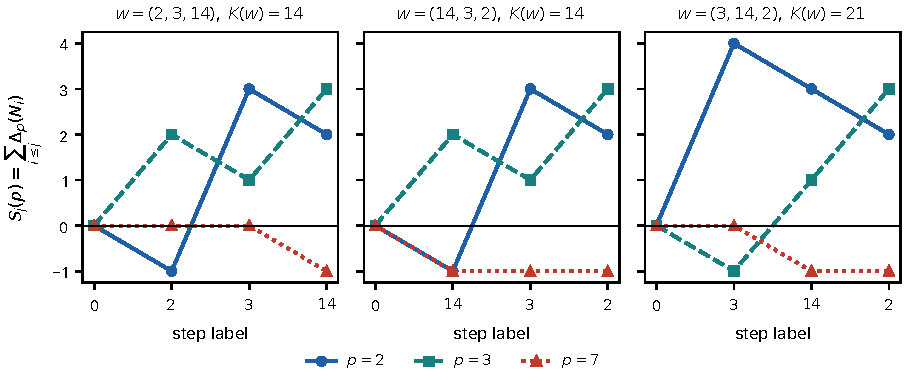
\includegraphics[width=\textwidth]{fig05_valuation_trajectories}
\caption{\textbf{Valuation trajectories of three words of the content $\{2,3,14\}$ (exact).} The curves are $S_j(p)$ for $p=2$ (solid, circles), $3$ (dashed, squares) and $7$ (dotted, triangles); $K(w)=\prod_pp^{\max(0,-\min_jS_j(p))}$ is printed above each panel: $14=2\cdot7$ for $(2,3,14)$ and $(14,3,2)$ (minima $-1$ at $p=2$ and $-1$ at $p=7$) and $21=3\cdot7$ for $(3,14,2)$. Theorem illustrated: \cref{thm:threshold}.}\label{fig:valuation}
\end{figure}
\begin{figure}[tbp]\centering
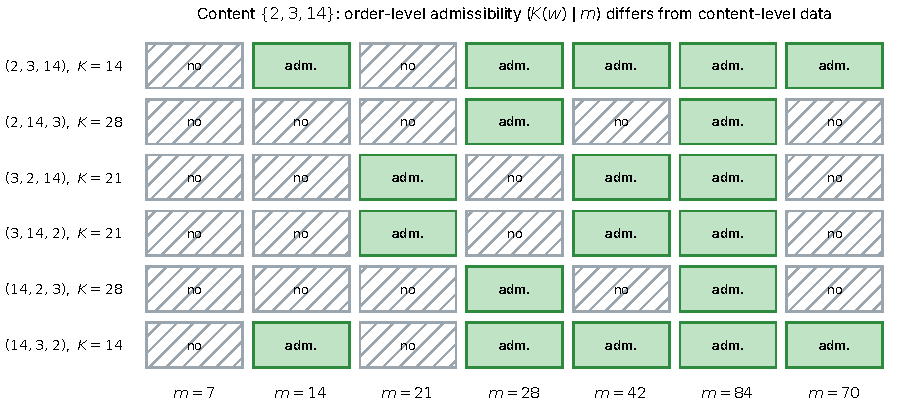
\includegraphics[width=\textwidth]{fig06_content_vs_order}
\caption{\textbf{Content-level versus order-level admissibility for $\{2,3,14\}$ (exact).} Rows: the six arrangements with their thresholds $K$; columns: sources. A cell is filled and marked ``adm.'' iff $K\mid m$. The same content is wholly inadmissible at $m=7$, partly admissible at $m=14$ and $m=21$, and fully admissible among the sources shown only at $m=84=P(C)$ (\cref{prop:sat}); it is connected for $m=28$ (\cref{thm:2314}) although $84\nmid28$.}\label{fig:content}
\end{figure}
